\documentclass{amsart}
\usepackage{tikz}
\usepackage{chessboard}
\author{David Prentiss}
\date{\today}
\title{Homework 1}
\begin{document}
\maketitle

\section{}
There are 6 teams in the football league: Vultures (V), Lions (L), Eagles (E),
Beavers (B), Terps (T) and Skunks (S).
The V's have already played the L's and the E's; the L's have also played the
B's \& S's.
The T's have played the E's and S's. Each team plays one game per week.
Find a schedule so that all teams will have played each other in the fewest
number of weeks.
Hint: Create a graph whose vertices are the pairs of teams that have not yet
played each other.
What should the edges be so that in a legal coloring of the graph each color can
represent the games played in one week?
Give a solution and show that it is optimal.

\subsubsection*{Solution}
To find an optimal schedule for the remaining league games, begin by creating a
graph with teams as vertices and edges representing completed games.
The edges of this graph's compliment represents games that must be scheduled.
Figure \ref{fig:teams} shows both graphs.
\begin{figure}[!h]
  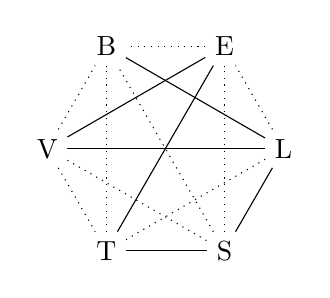
\begin{tikzpicture}
    \foreach [count=\i] \team in {B, E, L, S, T, V} {
      \node (\team) at (-60*\i+180:1.5cm) {\team};
    }
    \draw (T) -- (S);
    \draw (L) -- (B);
    \draw (V) -- (L);
    \draw (V) -- (E);
    \draw (L) -- (S);
    \draw (T) -- (E);
    \draw[dotted] (V) -- (B);
    \draw[dotted] (V) -- (T);
    \draw[dotted] (V) -- (S);
    \draw[dotted] (S) -- (E);
    \draw[dotted] (S) -- (B);
    \draw[dotted] (L) -- (T);
    \draw[dotted] (L) -- (E);
    \draw[dotted]  (T) -- (B);
    \draw[dotted]  (E) -- (B);
  \end{tikzpicture}
  \caption{A graph representing the league games thus far. A solid edge
    indicates the two teams have already played each other, while a dotted edge
    indicates a game between two teams that must be scheduled.}
  \label{fig:teams}
\end{figure}

From the compliment, construct a new graph with vertices representing games that
must be scheduled and edges representing matches that can not be scheduled
together.
From this graph we can see that the maximal clique size is four.
So, any legal 4-coloring of this graph represents an optimal weekly schedule.
See Figure \ref{fig:games}.
\begin{figure}[!h]
  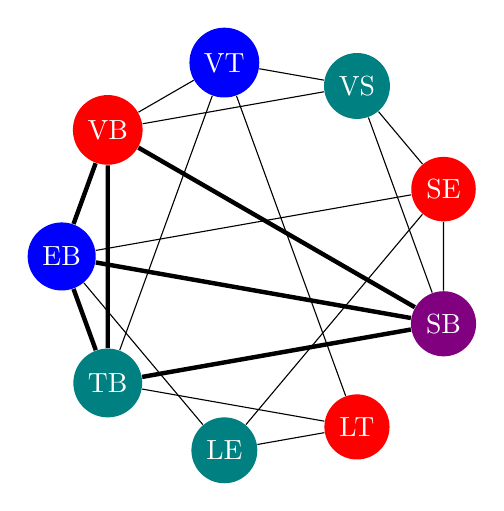
\begin{tikzpicture}
    \node[fill=red, text=white, circle] (VB) at (-40*1+180:2.5cm) {VB};
    \node[fill=blue, text=white, circle] (VT) at (-40*2+180:2.5cm) {VT};
    \node[fill=teal, text=white, circle] (VS) at (-40*3+180:2.5cm) {VS};
    \node[fill=red, text=white, circle] (SE) at (-40*4+180:2.5cm) {SE};
    \node[fill=violet, text=white, circle] (SB) at (-40*5+180:2.5cm) {SB};
    \node[fill=red, text=white, circle] (LT) at (-40*6+180:2.5cm) {LT};
    \node[fill=teal, text=white, circle] (LE) at (-40*7+180:2.5cm) {LE};
    \node[fill=teal, text=white, circle] (TB) at (-40*8+180:2.5cm) {TB};
    \node[fill=blue, text=white, circle] (EB) at (-40*9+180:2.5cm) {EB};

    %\draw (VB) -- (SE);
    %\draw[blue] (VB) -- (LT);
    %\draw (VB) -- (LE);
    %\draw (VT) -- (SE);
    %\draw (VT) -- (SB);
    %\draw (VT) -- (LE);
    %\draw (VT) -- (EB);
    %\draw[teal] (VS) -- (LT);
    %\draw (VS) -- (LE);
    %\draw (VS) -- (TB);
    %\draw (VS) -- (EB);
    %\draw[red] (SE) -- (LT);
    %\draw (SE) -- (TB);
    %\draw (SE) -- (TB);
    %\draw[violet] (SB) -- (LT);
    %\draw (SB) -- (LE);
    %\draw[orange] (LT) -- (EB);
    %\draw (LE) -- (TB);

    \draw (VB) -- (VT) -- (VS) -- (VB);
    \draw (VS) -- (SE) -- (SB) -- (VS);
    \draw (LT) -- (LE);
    \draw (VT) -- (LT) -- (TB) -- (VT);
    \draw (SE) -- (LE) -- (EB) -- (SE);
    \draw[ultra thick] (VB) -- (SB) -- (TB) -- (EB) -- (VB) -- (TB);
    \draw[ultra thick] (SB) -- (EB);
  \end{tikzpicture}
  \caption{A graph coloring representing an optimal schedule for the remaining
    league games.
    Edges connect matches that cannot occur in the same week.
    Vertices with the same color represent matches that may be scheduled in the
    same same week.
    Thick edges connect a maximal clique.
    }
    \label{fig:games}
\end{figure}

\section{} %2

(i) Show that in a nondirected graph $G$, the independence number of $G$ is less
than the dominance number of $G$, by showing that every maximal independent
set is a dominating set.
\subsubsection*{Solution}
For any graph, a maximal independent set of vertices is a dominating set.
\begin{proof}
  If an independent set is maximal, then by definition, there are no other
  independent vertices that could be added.
  This set must also be a dominating set since, if there were any vertices not
  adjacent to it, they would be independent, and therefore the previous set could
  not have been maximal.
\end{proof}

(ii) Give an example to show that the minimum dominating set is not necessarily
independent.
\subsubsection*{Solution}
Consider the graphs in Figure 3.
\begin{figure}[!h]
  \begin{tikzpicture}
    \draw (0,0) node[circle, fill=black, draw] -- (1,0) node[circle, fill=red, draw]
    -- (2,0) node[circle, fill=red,draw] -- (3,0) node[circle, fill=black, draw];
    \draw (0,1) node[circle, fill=red, draw] -- (1,1) node[circle, fill=black]
    -- (2,1) node[circle, fill=black] -- (3,1) node[circle, fill=red, draw];
  \end{tikzpicture}
  \label{fig:mindom}
  \caption{
The red vertices in both graphs are minimum dominating sets, but the upper set is independent while
the lower one is not.}
\end{figure}

\section{}

Let $P_1$ and $P_2$ be two paths in a graph $G$, and let $G^\prime=P_1 \cap P_2$ possess at least 2
vertices.
Show that if $G^\prime$ is disconnected then $P_1\cup P_2$ contains a cycle.

\section{}
A bipartite graph is given by the following adjacency list: a-1,2,5; b-1,3; c-2-3-5; d-4,5; e2,5,6; f-5,6.

\begin{figure}[!h]
  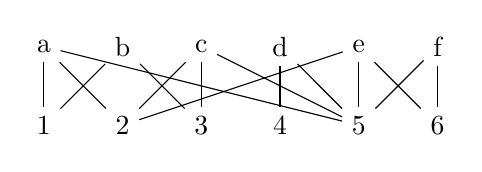
\begin{tikzpicture}
    \foreach [count=\i] \letter in {a, b, c, d, e, f} {
      \node (\letter) at (\i, 1) {\letter};
      \node (\i) at (\i, 0) {\i};
    }
    \draw (a) -- (1);
    \draw (a) -- (2);
    \draw (a) -- (5);
    \draw (b) -- (1);
    \draw (b) -- (3);
    \draw (c) -- (2);
    \draw (c) -- (3);
    \draw (c) -- (5);
    \draw (d) -- (4);
    \draw (d) -- (5);
    \draw (e) -- (2);
    \draw (e) -- (5);
    \draw (e) -- (6);
    \draw (f) -- (5);
    \draw (f) -- (6);
  \end{tikzpicture}
\end{figure}
\subsection*{a.}
Find the minimum vertex coloring. Prove that your solution is optimal.
\subsubsection*{Solution}
Let the above graph be graph $G$.
Since $G$ is bipartite, then by definition its vertices can be divided into two
disjoint sets such that no two edges in the same set are adjacent.
Since none of the edges in a set are adjacent, each set may be assigned a single
color and the graph will require at most two colors.
Therefore, since $G$ bipartite and not empty, it is 2-chromatic.
\begin{figure}[h]
  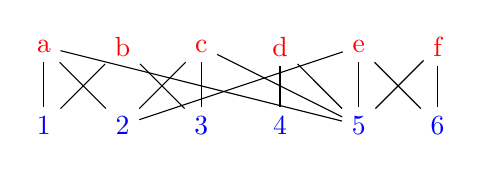
\begin{tikzpicture}
    \foreach [count=\i] \letter in {a, b, c, d, e, f} {
      \node[red] (\letter) at (\i, 1) {\letter};
      \node[blue] (\i) at (\i, 0) {\i};
    }
    \draw (a) -- (1);
    \draw (a) -- (2);
    \draw (a) -- (5);
    \draw (b) -- (1);
    \draw (b) -- (3);
    \draw (c) -- (2);
    \draw (c) -- (3);
    \draw (c) -- (5);
    \draw (d) -- (4);
    \draw (d) -- (5);
    \draw (e) -- (2);
    \draw (e) -- (5);
    \draw (e) -- (6);
    \draw (f) -- (5);
    \draw (f) -- (6);
  \end{tikzpicture}
\end{figure}

In a sense, $G$ is already two-colored in that the vertices $\{1,2,3,4,5,6\}$
are labeled with numerals while
$\{\text{a},\text{b},\text{c},\text{d},\text{e},\text{f}\}$
are labeled with letters.
However, while all bipartite graphs are 2-colorable, it is not the case that
they necessarily have a unique 2-coloring.
Consider $G$ for example, if the edge connecting nodes \{d\} and \{5\} were
removed, then the resulting subgraph containing \{d\} and \{4\} would
no longer be connected and we would have our choice of either coloring.
That is, (\{d\},\{4\}) or (\{4\},\{d\}).


\subsection*{b.}
Find the minimum edge coloring. What is a simple lower bound for the edge coloring of a
graph? Use this to prove that your solution is optimal.
\subsubsection*{Solution}
Since the order of vertex ``5'' is 5, any 5-coloring is a minimal edge coloring.
\begin{figure}[!h]
  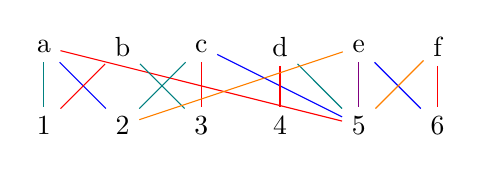
\begin{tikzpicture}
    \foreach [count=\i] \letter in {a, b, c, d, e, f} {
      \node (\letter) at (\i, 1) {\letter};
      \node (\i) at (\i, 0) {\i};
    }
    \draw[teal] (a) -- (1);
    \draw[blue] (a) -- (2);
    \draw[red] (a) -- (5);
    \draw[red] (b) -- (1);
    \draw[teal] (b) -- (3);
    \draw[teal] (c) -- (2);
    \draw[red] (c) -- (3);
    \draw[blue] (c) -- (5);
    \draw[red] (d) -- (4);
    \draw[teal] (d) -- (5);
    \draw[orange] (e) -- (2);
    \draw[violet] (e) -- (5);
    \draw[blue] (e) -- (6);
    \draw[orange] (f) -- (5);
    \draw[red] (f) -- (6);
  \end{tikzpicture}
\end{figure}
\subsection*{c.}
Find a maximum matching. What is a simple upper bound to a maximum matching in a
graph? Use this to prove your solution is optimal.
\subsubsection*{Solution}
\begin{figure}[h]
  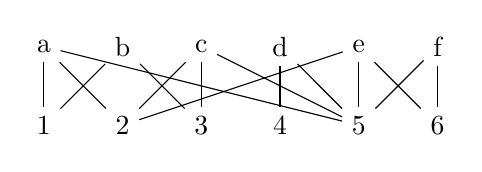
\begin{tikzpicture}
    \foreach [count=\i] \letter in {a, b, c, d, e, f} {
      \node (\letter) at (\i, 1) {\letter};
      \node (\i) at (\i, 0) {\i};
    }
    \draw (a) -- (1);
    \draw (a) -- (2);
    \draw (a) -- (5);
    \draw (b) -- (1);
    \draw (b) -- (3);
    \draw (c) -- (2);
    \draw (c) -- (3);
    \draw (c) -- (5);
    \draw (d) -- (4);
    \draw (d) -- (5);
    \draw (e) -- (2);
    \draw (e) -- (5);
    \draw (e) -- (6);
    \draw (f) -- (5);
    \draw (f) -- (6);
  \end{tikzpicture}
\end{figure}
\subsection*{d.}
Find a minimum edge cover. Prove that your solution is optimal.
\subsubsection*{Solution}
\begin{figure}[h]
  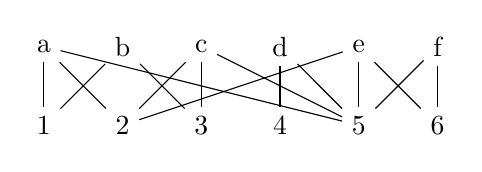
\begin{tikzpicture}
    \foreach [count=\i] \letter in {a, b, c, d, e, f} {
      \node (\letter) at (\i, 1) {\letter};
      \node (\i) at (\i, 0) {\i};
    }
    \draw (a) -- (1);
    \draw (a) -- (2);
    \draw (a) -- (5);
    \draw (b) -- (1);
    \draw (b) -- (3);
    \draw (c) -- (2);
    \draw (c) -- (3);
    \draw (c) -- (5);
    \draw (d) -- (4);
    \draw (d) -- (5);
    \draw (e) -- (2);
    \draw (e) -- (5);
    \draw (e) -- (6);
    \draw (f) -- (5);
    \draw (f) -- (6);
  \end{tikzpicture}
\end{figure}
\subsection*{e.}
Find a minimum vertex cover.
\subsubsection*{Solution}
\begin{figure}[h]
  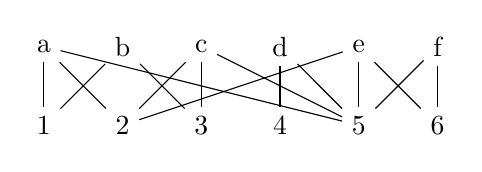
\begin{tikzpicture}
    \foreach [count=\i] \letter in {a, b, c, d, e, f} {
      \node (\letter) at (\i, 1) {\letter};
      \node (\i) at (\i, 0) {\i};
    }
    \draw (a) -- (1);
    \draw (a) -- (2);
    \draw (a) -- (5);
    \draw (b) -- (1);
    \draw (b) -- (3);
    \draw (c) -- (2);
    \draw (c) -- (3);
    \draw (c) -- (5);
    \draw (d) -- (4);
    \draw (d) -- (5);
    \draw (e) -- (2);
    \draw (e) -- (5);
    \draw (e) -- (6);
    \draw (f) -- (5);
    \draw (f) -- (6);
  \end{tikzpicture}
\end{figure}
\subsection*{f.}
Find a maximum independent set. Prove optimality of your solution.
\subsubsection*{Solution}
\begin{figure}[h]
  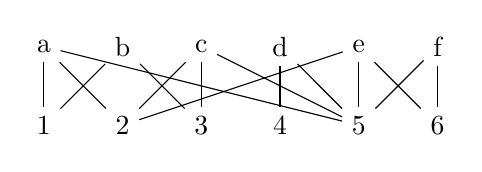
\begin{tikzpicture}
    \foreach [count=\i] \letter in {a, b, c, d, e, f} {
      \node (\letter) at (\i, 1) {\letter};
      \node (\i) at (\i, 0) {\i};
    }
    \draw (a) -- (1);
    \draw (a) -- (2);
    \draw (a) -- (5);
    \draw (b) -- (1);
    \draw (b) -- (3);
    \draw (c) -- (2);
    \draw (c) -- (3);
    \draw (c) -- (5);
    \draw (d) -- (4);
    \draw (d) -- (5);
    \draw (e) -- (2);
    \draw (e) -- (5);
    \draw (e) -- (6);
    \draw (f) -- (5);
    \draw (f) -- (6);
  \end{tikzpicture}
\end{figure}

\section{}
In a given connected graph with specified arc weights, suppose there exists an arc whose
weight is smaller than that of any other in G. Prove that this arc must be contained in every
minimum spanning tree in G.
\subsubsection*{Solution}

\section{}
Show that for any graph, $G$, the number of vertices with odd degree is even.
\begin{proof}
  Consider an empty graph with at least two vertices.
  All vertices are order zero.
  If an edge is added to the graph, then exactly two of the vertices have order
  one.
  These, vertices have odd degree and there is an even number.

  Now consider an incomplete graph $G$ with $k$ vertices.
  Every vertex is either odd, even, or disconnected (order zero).
  If a new edge is added to the graph, there are the following three
  possibilities
  \begin{enumerate}
  \item the edge is added between two vertices with even degree or degree zero,
  \item the edge is added between two odd vertices, or
  \item the edge is added between one oven and one odd vertex.
  \end{enumerate}
  In case one, two new vertices of odd degree are created.
  In case two, the number of odd vertices in decreased by two.
  Int case three, the even vertex becomes odd, the odd vertex becomes even, and
  the number of odd vertices is unchanged.

  Since a graph with one edge (and trivially zero edges) has an even number of
  odd vertices, and adding any new edges to a graph adds or removes two (or
  zero) new edges, then it is not possible to construct a graph with an odd
  number of odd vertices.
\end{proof}

\section{}
Is it possible for a cutset and a cycle to contain exactly one edge in common? Why?
\subsubsection*{Solution}

\section{}
Suppose forest $F$ consists of $t$ trees and contains $v$ vertices. How many
edges are in forest $F$?

\subsubsection*{Solution}

A forest, $F$, of $t$ trees and $v$ vertices has $v-t$ edges.
\begin{proof}
  Remember that for a tree, $T_i$, with $v_i$ vertices, the number of edges,
  $e_i$, is $v_i - 1$ edges.
  For forest $F$ with trees $\{T_1, T_2,...,T_t\}$, the number of vertices is
  \begin{equation}
    v = \sum_{i=1}^t v_i.
  \end{equation}
  The number of edges, then, is
  \begin{equation}
    \sum_{i=1}^t e_i = \sum_{i=1}^t v_i -1 = \sum_{i=1}^t v_i - \sum_{i=1}^t  1 = v - t.
  \end{equation}
\end{proof}

\section{} %9
A classic problem is the ``knight's tour.''
On an $n \times n$ chessboard, starting from some
square, move the knight so that it lands on every space exactly once.
Show how a graph can be used to solve this problem.
Illustrate on a 4 by 4 chessboard.

\subsubsection*{Solution}
The knight's tour is equivalent to a Hamiltonian path. This may be illustrated
by a graph who's vertices are the spaces on the chessboard and the edges connect
spaced that are adjacent with respect to possible knight moves.

\begin{figure}[h]
  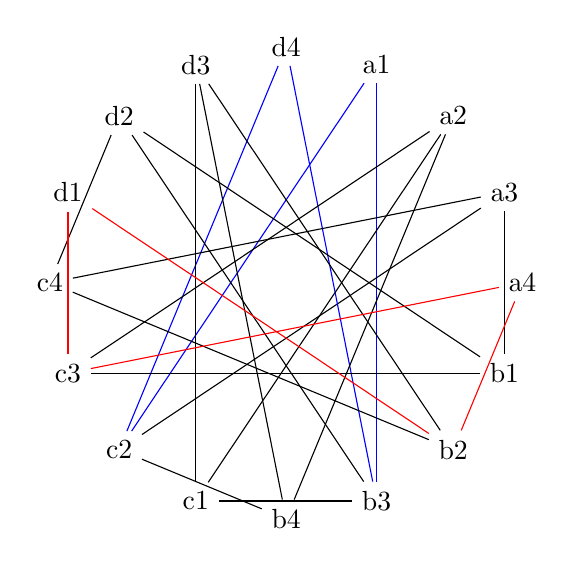
\begin{tikzpicture}
    \foreach [count=\i] \row in {1, 2, 3, 4} {
      \foreach [count=\j] \col in {a, b, c, d} {
       \node (\col\row) at ({-360/16*(\i+(4*\j))+180}:3cm) {\col\row};
      }
    }
    \draw[blue] (a1) -- (c2);
    \draw[blue] (a1) -- (b3);
    \draw (c2) -- (a3);
    \draw (c2) -- (b4);
    \draw[blue] (c2) -- (d4);
    \draw[blue] (b3) -- (d4);
    \draw (b3) -- (d2);
    \draw (b3) -- (c1);
    \draw (a3) -- (b1);
    \draw (a3) -- (c4);
    \draw (b4) -- (a2);
    \draw (b4) -- (d3);
    \draw (d2) -- (b1);
    \draw (d2) -- (c4);
    \draw (c1) -- (a2);
    \draw (c1) -- (d3);
    \draw (b1) -- (c3);
    \draw (c4) -- (b2);
    \draw (a2) -- (c3);
    \draw (d3) -- (b2);
    \draw[red] (c3) -- (a4);
    \draw[red] (c3) -- (d1);
    \draw[red] (b2) -- (a4);
    \draw[red] (b2) -- (d1);
  \end{tikzpicture}
  \caption{}
\end{figure}

\section{}
Show how to use a graph to solve the following puzzle. Place the numbers 1 through 8 in the
boxes so that no two consecutive numbers are horizontally, vertically, or diagonally adjacent
to each other.
\begin{figure}[h!]
  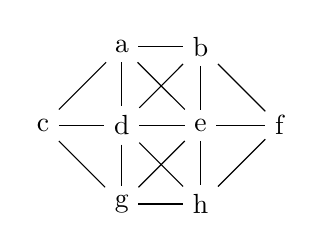
\begin{tikzpicture}
    \node (a) at (1, 2) {a};
    \node (b) at (2, 2) {b};
    \node (c) at (0, 1) {c};
    \node (d) at (1, 1) {d};
    \node (e) at (2, 1) {e};
    \node (f) at (3, 1) {f};
    \node (g) at (1, 0) {g};
    \node (h) at (2, 0) {h};
    \draw (a) -- (b);
    \draw (a) -- (c);
    \draw (a) -- (d);
    \draw (a) -- (e);
    \draw (b) -- (d);
    \draw (b) -- (e);
    \draw (b) -- (f);
    \draw (c) -- (d);
    \draw (c) -- (g);
    \draw (d) -- (e);
    \draw (d) -- (g);
    \draw (d) -- (h);
    \draw (e) -- (f);
    \draw (e) -- (g);
    \draw (e) -- (h);
    \draw (f) -- (h);
    \draw (g) -- (h);
  \end{tikzpicture}
  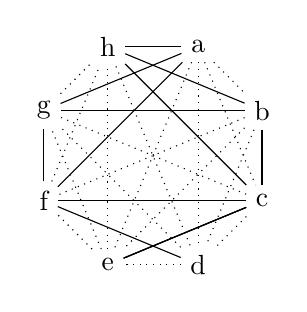
\begin{tikzpicture}
    \foreach [count=\i] \cell in {a, b, c, d, e, f, g, h} {
      \node (\cell) at (-360/8*\i+112.5:1.5cm) {\cell};
    }
    \draw (a) -- (f);
    \draw (a) -- (g);
    \draw (a) -- (h);
    \draw (b) -- (c);
    \draw (b) -- (g);
    \draw (b) -- (h);
    \draw (c) -- (b);
    \draw (c) -- (e);
    \draw (c) -- (f);
    \draw (c) -- (h);
    \draw (d) -- (f);
    \draw (e) -- (c);
    \draw (e) -- (c);
    \draw (f) -- (g);
    \draw (f) -- (g);

    \draw[dotted] (a) -- (b);
    \draw[dotted] (a) -- (c);
    \draw[dotted] (a) -- (d);
    \draw[dotted] (a) -- (e);
    \draw[dotted] (b) -- (d);
    \draw[dotted] (b) -- (e);
    \draw[dotted] (b) -- (f);
    \draw[dotted] (c) -- (d);
    \draw[dotted] (c) -- (g);
    \draw[dotted] (d) -- (e);
    \draw[dotted] (d) -- (g);
    \draw[dotted] (d) -- (h);
    \draw[dotted] (e) -- (f);
    \draw[dotted] (e) -- (g);
    \draw[dotted] (e) -- (h);
    \draw[dotted] (f) -- (h);
    \draw[dotted] (g) -- (h);
  \end{tikzpicture}
  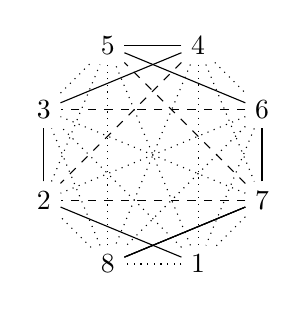
\begin{tikzpicture}
    \node (a) at (-360/8*1+112.5:1.5cm) {4};
    \node (b) at (-360/8*2+112.5:1.5cm) {6};
    \node (c) at (-360/8*3+112.5:1.5cm) {7};
    \node (d) at (-360/8*4+112.5:1.5cm) {1};
    \node (e) at (-360/8*5+112.5:1.5cm) {8};
    \node (f) at (-360/8*6+112.5:1.5cm) {2};
    \node (g) at (-360/8*7+112.5:1.5cm) {3};
    \node (h) at (-360/8*8+112.5:1.5cm) {5};

    \draw[dashed] (a) -- (f);
    \draw (a) -- (g);
    \draw (a) -- (h);
    \draw (b) -- (c);
    \draw[dashed] (b) -- (g);
    \draw (b) -- (h);
    \draw (c) -- (b);
    \draw (c) -- (e);
    \draw[dashed] (c) -- (f);
    \draw[dashed] (c) -- (h);
    \draw (d) -- (f);
    \draw (e) -- (c);
    \draw (e) -- (c);
    \draw (f) -- (g);
    \draw (f) -- (g);

    \draw[dotted] (a) -- (b);
    \draw[dotted] (a) -- (c);
    \draw[dotted] (a) -- (d);
    \draw[dotted] (a) -- (e);
    \draw[dotted] (b) -- (d);
    \draw[dotted] (b) -- (e);
    \draw[dotted] (b) -- (f);
    \draw[dotted] (c) -- (d);
    \draw[dotted] (c) -- (g);
    \draw[dotted] (d) -- (e);
    \draw[dotted] (d) -- (g);
    \draw[dotted] (d) -- (h);
    \draw[dotted] (e) -- (f);
    \draw[dotted] (e) -- (g);
    \draw[dotted] (e) -- (h);
    \draw[dotted] (f) -- (h);
    \draw[dotted] (g) -- (h);
  \end{tikzpicture}
  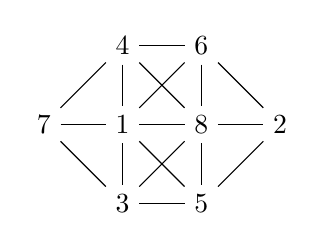
\begin{tikzpicture}
    \node (a) at (1, 2) {4};
    \node (b) at (2, 2) {6};
    \node (c) at (0, 1) {7};
    \node (d) at (1, 1) {1};
    \node (e) at (2, 1) {8};
    \node (f) at (3, 1) {2};
    \node (g) at (1, 0) {3};
    \node (h) at (2, 0) {5};
    \draw (a) -- (b);
    \draw (a) -- (c);
    \draw (a) -- (d);
    \draw (a) -- (e);
    \draw (b) -- (d);
    \draw (b) -- (e);
    \draw (b) -- (f);
    \draw (c) -- (d);
    \draw (c) -- (g);
    \draw (d) -- (e);
    \draw (d) -- (g);
    \draw (d) -- (h);
    \draw (e) -- (f);
    \draw (e) -- (g);
    \draw (e) -- (h);
    \draw (f) -- (h);
    \draw (g) -- (h);
  \end{tikzpicture}
  \caption{}
\end{figure}


\end{document}

\draw[blue] (a1) -- (c2);
\draw[blue] (a1) -- (b3);
\draw[blue] (c2) -- (a3);
\draw[blue] (c2) -- (b4);
\draw[blue] (c2) -- (d4);
\draw[blue] (b3) -- (d4);
\draw[blue] (b3) -- (d2);
\draw[blue] (b3) -- (c1);
\draw[blue] (a3) -- (b1);
\draw[blue] (a3) -- (c4);
\draw[blue] (b4) -- (a2);
\draw[blue] (b4) -- (d3);
\draw[blue] (d2) -- (b1);
\draw[blue] (d2) -- (c4);
\draw[blue] (c1) -- (a2);
\draw[blue] (c1) -- (d3);
\draw[blue] (b1) -- (c3);
\draw[blue] (c4) -- (b2);
\draw[blue] (a2) -- (c3);
\draw[blue] (a2) -- (c3);
\draw[blue] (d3) -- (b2);